\documentclass[portrait,final,a1paper,fontscale=0.4]{baposter}

\usepackage{calc}
\usepackage{graphicx}
\usepackage{amsmath}
\usepackage{amssymb}
\usepackage{relsize}
\usepackage{multirow}
\usepackage{rotating}
\usepackage{bm}
\usepackage{enumitem}
\usepackage[hyphens]{url}
\usepackage{booktabs}
\usepackage{subfigure}
\usepackage{graphicx}
\usepackage{multicol}

%\usepackage{times}
%\usepackage{helvet}
%\usepackage{bookman}
\usepackage{palatino}
\usepackage{pgf}
\usepackage{tikz}
\usetikzlibrary{shapes}
\usepackage{PGFTikzGraph}
\newcommand{\captionfont}{\footnotesize}

\graphicspath{{images/}{../images/}}
\usetikzlibrary{calc}


\newcommand{\Matrix}[1]{\begin{bmatrix} #1 \end{bmatrix}}
\newcommand{\Vector}[1]{\begin{pmatrix} #1 \end{pmatrix}}

\newcommand*{\norm}[1]{\mathopen\| #1 \mathclose\|}% use instead of $\|x\|$
\newcommand*{\abs}[1]{\mathopen| #1 \mathclose|}% use instead of $\|x\|$
\newcommand*{\normLR}[1]{\left\| #1 \right\|}% use instead of $\|x\|$

\newcommand*{\SET}[1]  {\ensuremath{\mathcal{#1}}}
\newcommand*{\FUN}[1]  {\ensuremath{\mathcal{#1}}}
\newcommand*{\MAT}[1]  {\ensuremath{\boldsymbol{#1}}}
\newcommand*{\VEC}[1]  {\ensuremath{\boldsymbol{#1}}}
\newcommand*{\CONST}[1]{\ensuremath{\mathit{#1}}}

\DeclareMathOperator*{\argmax}{arg\,max}
\DeclareMathOperator*{\diag}{diag}
\DeclareMathOperator*{\argmin}{arg\,min}
\DeclareMathOperator*{\vectorize}{vec}
\DeclareMathOperator*{\reshape}{reshape}

%\font\dsfnt=dsrom12

\newcommand{\SNN}{\ensuremath{\mathbb N}}
\newcommand{\SRR}{\ensuremath{\mathbb R}}
\newcommand{\SZZ}{\ensuremath{\mathbb Z}}
%-----------------------------------------------------------------------------
% Matrices of the shape model
\renewcommand{\a}{\VEC\alpha}
\renewcommand{\v}{\VEC v}
\renewcommand{\l}{\VEC l}
\newcommand*{\m}{\VEC{\mu}}
\newcommand*{\M}{\MAT{M}}
\renewcommand*{\P}{\MAT{\Pi}}

%\newcommand{\J}{\SET J}
\newcommand{\J}{\SET{P}}
\newcommand{\Active}{\mathcal{A}}
\newcommand{\Selection}{\mathbf{S}}
\newcommand{\AllSelections}{\mathfrak{S}}
\newcommand{\Params}{\VEC\Theta}

%%%%%%%%%%%%%%%%%%%%%%%%%%%%%%%%%%%%%%%%%%%%%%%%%%%%%%%%%%%%%%%%%%%%%%%%%%%%%%%%
%%%% Some math symbols used in the text
%%%%%%%%%%%%%%%%%%%%%%%%%%%%%%%%%%%%%%%%%%%%%%%%%%%%%%%%%%%%%%%%%%%%%%%%%%%%%%%%

%%%%%%%%%%%%%%%%%%%%%%%%%%%%%%%%%%%%%%%%%%%%%%%%%%%%%%%%%%%%%%%%%%%%%%%%%%%%%%%%
% Multicol Settings
%%%%%%%%%%%%%%%%%%%%%%%%%%%%%%%%%%%%%%%%%%%%%%%%%%%%%%%%%%%%%%%%%%%%%%%%%%%%%%%%
\setlength{\columnsep}{1.5em}
\setlength{\columnseprule}{0mm}

%%%%%%%%%%%%%%%%%%%%%%%%%%%%%%%%%%%%%%%%%%%%%%%%%%%%%%%%%%%%%%%%%%%%%%%%%%%%%%%%
% Save space in lists. Use this after the opening of the list
%%%%%%%%%%%%%%%%%%%%%%%%%%%%%%%%%%%%%%%%%%%%%%%%%%%%%%%%%%%%%%%%%%%%%%%%%%%%%%%%
\newcommand{\compresslist}{%
\setlength{\itemsep}{1pt}%
\setlength{\parskip}{0pt}%
\setlength{\parsep}{0pt}%
}

%%%%%%%%%%%%%%%%%%%%%%%%%%%%%%%%%%%%%%%%%%%%%%%%%%%%%%%%%%%%%%%%%%%%%%%%%%%%%%
%%% Begin of Document
%%%%%%%%%%%%%%%%%%%%%%%%%%%%%%%%%%%%%%%%%%%%%%%%%%%%%%%%%%%%%%%%%%%%%%%%%%%%%%

\begin{document}

%%%%%%%%%%%%%%%%%%%%%%%%%%%%%%%%%%%%%%%%%%%%%%%%%%%%%%%%%%%%%%%%%%%%%%%%%%%%%%
%%% Here starts the poster
%%%---------------------------------------------------------------------------
%%% Format it to your taste with the options
%%%%%%%%%%%%%%%%%%%%%%%%%%%%%%%%%%%%%%%%%%%%%%%%%%%%%%%%%%%%%%%%%%%%%%%%%%%%%%
% Define some colors

\definecolor{lightorange}{rgb}{0.9,0.4,0}
\definecolor{lightestorange}{rgb}{1,0.8,0.5}
\definecolor{darkorange}{rgb}{0.2,0.1,0}
\definecolor{LightBrown}{rgb}{0.8,0.8,0.7}

\hyphenation{resolution occlusions}
%%
\begin{poster}%
  % Poster Options
  {
  columns=2,
  % Show grid to help with alignment
  grid=false,
  % Column spacing
  colspacing=1em,
  % Color style
  bgColorOne=white,
  bgColorTwo=white,
  borderColor=black,
  headerColorOne=black,
  headerColorTwo=black,
  headerFontColor=white,
  boxColorOne=black,
  boxColorTwo=LightBrown,
  % Format of textbox
  textborder=faded,
  % Format of text header
  eyecatcher=true,
  headerborder=closed,
  headerheight=0.1\textheight,
%  textfont=\sc, An example of changing the text font
  headershape=rectangle,
  headershade=shadelr,
  headerfont=\Large\bf\textsc, %Sans Serif
  textfont={\setlength{\parindent}{1.5em}},
  textborder=rectangle,
  boxshade=none,
%  background=shade-tb,
  background=plain,
  linewidth=2pt
  }
  % Eye Catcher
  { 
  \includegraphics[height=6.0em]{Figures/FigCh03_2DDNGSteadyStateLossy}
  } 
  % Title
  {\bf\textsc{Finite Difference Time--Domain Modelling of Metamaterials: GPU Implementation of Cylindrical Cloak}\vspace{0.4em}}
  % Authors
  {\textsc{Attique.Dawood@nu.edu.pk}\vspace{-0.8em}}
  % University logo
  {% The makebox allows the title to flow into the logo, this is a hack because of the L shaped logo.
  \includegraphics[height=7.0em]{Figures/NU_Logo_Text}
  %\hspace*{-1.675cm}
  %\centering
  %\raisebox{-1.0em}{\includegraphics[height=1.0em]{Figures/FAST-NU}}
  }

%%%%%%%%%%%%%%%%%%%%%%%%%%%%%%%%%%%%%%%%%%%%%%%%%%%%%%%%%%%%%%%%%%%%%%%%%%%%%%
%%% Now define the boxes that make up the poster
%%%---------------------------------------------------------------------------
%%% Each box has a name and can be placed absolutely or relatively.
%%% The only inconvenience is that you can only specify a relative position 
%%% towards an already declared box. So if you have a box attached to the 
%%% bottom, one to the top and a third one which should be in between, you 
%%% have to specify the top and bottom boxes before you specify the middle 
%%% box.
%%%%%%%%%%%%%%%%%%%%%%%%%%%%%%%%%%%%%%%%%%%%%%%%%%%%%%%%%%%%%%%%%%%%%%%%%%%%%%
    %
    % A coloured circle useful as a bullet with an adjustably strong filling
    \newcommand{\colouredcircle}{%
      \tikz{\useasboundingbox (-0.2em,-0.32em) rectangle(0.2em,0.32em); \draw[draw=black,fill=lightblue,line width=0.03em] (0,0) circle(0.18em);}}

%%%%%%%%%%%%%%%%%%%%%%%%%%%%%%%%%%%%%%%%%%%%%%%%%%%%%%%%%%%%%%%%%%%%%%%%%%%%%%
  \headerbox{Abstract}{name=abstract,column=0,row=0}{
%%%%%%%%%%%%%%%%%%%%%%%%%%%%%%%%%%%%%%%%%%%%%%%%%%%%%%%%%%%%%%%%%%%%%%%%%%%%%%
  Finite difference time--domain (FDTD) technique can be used to model metamaterials by treating them as dispersive material. Drude or Lorentz model can be incorporated into the standard FDTD algorithm for modelling negative permittivity and permeability.
  
  FDTD algorithm is readily parallelisable and can take advantage of GPU acceleration achieving speed--ups of 5x--50x depending on hardware setup. \textbf{Metamaterial scattering problems are implemented using dispersive FDTD technique on GPU resulting in performance gain of 10x--15x compared to conventional CPU implementation}.
 }

%%%%%%%%%%%%%%%%%%%%%%%%%%%%%%%%%%%%%%%%%%%%%%%%%%%%%%%%%%%%%%%%%%%%%%%%%%%%%%
  \headerbox{Drude Dispersive Model}{name=drude,column=0,below=abstract}{
%%%%%%%%%%%%%%%%%%%%%%%%%%%%%%%%%%%%%%%%%%%%%%%%%%%%%%%%%%%%%%%%%%%%%%%%%%%%%%
 A material is dispersive\index{dispersive material} if its permittivity or permeability is dependent on frequency~\cite[Ch. 10]{JBSchneiderUFDTD}.
  
  The relative permittivity in Drude model\index{Drude model $\epsilon_r(\omega)$} is given by
  \begin{equation}
  \centering
  \hat{\epsilon_r}(\omega)=\epsilon_\infty-\dfrac{\omega^2_p}{\omega^2-j\gamma\omega}.
  \label{er-Drude}
  \end{equation}
  Where, $\omega_p$ is plasma frequency and $\gamma$ is collision frequency. Setting $\gamma=0$ and $\epsilon_\infty=1$, relative permittivity comes out to be negative for $\omega/\omega_p > 1$. Thus, Drude model can be effectively used to model metamaterials\index{metamaterial} with permittivity or permeability less than one by incorporating it into FDTD update equations.
  }

%%%%%%%%%%%%%%%%%%%%%%%%%%%%%%%%%%%%%%%%%%%%%%%%%%%%%%%%%%%%%%%%%%%%%%%%%%%%%%
\headerbox{Problem Geometry}{name=geometry,column=1,span=1,row=0}
{
\centering
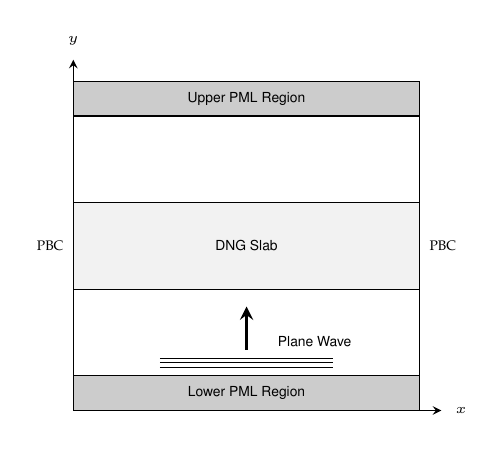
\begin{tikzpicture}[xscale=0.55,yscale=0.55,font=\tiny]
	\newcommand{\LeftX}{0cm}
	\newcommand{\MidX}{4cm}
	\newcommand{\RightX}{8cm}
	\newcommand{\PMLw}{0.8cm}
	\newcommand{\DomainY}{6.0cm}
	\newcommand{\SlabStartY}{2.0cm+\PMLw}
	\newcommand{\SlabEndY}{4.0cm+\PMLw}
	% x-axis.
	\draw[->, >=stealth] (\LeftX,0cm) -- (\RightX+0.5cm,0cm);
	\coordinate [label=right:$x$] (x-axis) at (\RightX+0.6cm,0cm);
	% y-axis.
	\draw[->, >=stealth] (\LeftX,0cm) -- (\LeftX,2*\PMLw+\DomainY+0.5cm);
	\coordinate [label=above:$y$] (y-axis) at (\LeftX,2*\PMLw+\DomainY+0.6cm);
	% PBCs.
	\coordinate [label=right:PBC] (PBCright) at (\RightX,\PMLw+3.0cm);
	\coordinate [label=left:PBC] (PBCleft) at (\LeftX,\PMLw+3.0cm);
	% Lower PML Region.
	\draw[fill=gray!40!white] (\LeftX,0cm) rectangle (\RightX,\PMLw);
	\coordinate [label=center:\textsf{Lower PML Region}] (LowerPML) at (\MidX,0.4cm);
	% Solution Region.
	\draw (\LeftX,\PMLw) rectangle (\RightX,\PMLw+\DomainY);
	% Upper PML Region.
	\draw[fill=gray!40!white] (\LeftX,\PMLw+\DomainY) rectangle (\RightX,2*\PMLw+\DomainY);
	\coordinate [label=center:\textsf{Upper PML Region}] (UpperPML) at (\MidX,\PMLw+\DomainY+0.4cm);
	% Slab.
	\draw[fill=gray!10!white] (\LeftX,\SlabStartY) rectangle (\RightX,\SlabEndY);
	\coordinate [label=center:\textsf{DNG Slab}] (DNGSlab) at (\MidX,\PMLw+3.0cm);
	% Plane wave.
	\draw (\LeftX+2.0cm,\PMLw+0.2cm) -- (\RightX-2.0cm, \PMLw+0.2cm);
	\draw (\LeftX+2.0cm,\PMLw+0.3cm) -- (\RightX-2.0cm, \PMLw+0.3cm);
	\draw (\LeftX+2.0cm,\PMLw+0.4cm) -- (\RightX-2.0cm, \PMLw+0.4cm);
	\draw[line width=1.1pt, ->, >=stealth] (\MidX,\PMLw+0.6cm) -- (\MidX,\PMLw+1.6cm);
	\coordinate [label=right:\textsf{Plane Wave}] (PlaneWave) at (\MidX+0.5cm,\PMLw+0.8cm);
\end{tikzpicture}
\centering
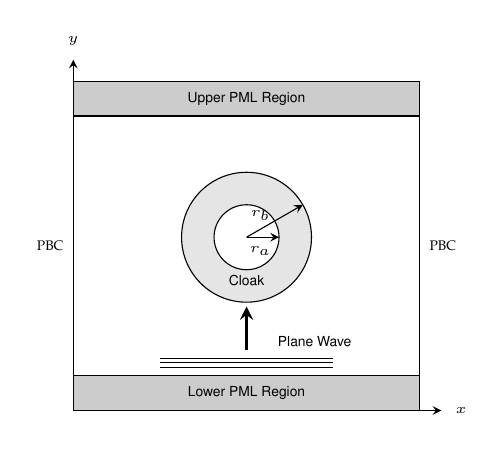
\begin{tikzpicture}[xscale=0.55,yscale=0.55,font=\tiny]
	\newcommand{\LeftX}{0cm}
	\newcommand{\MidX}{4cm}
	\newcommand{\RightX}{8cm}
	\newcommand{\PMLw}{0.8cm}
	\newcommand{\DomainY}{6.0cm}
	\newcommand{\SlabStartY}{2.0cm+\PMLw}
	\newcommand{\SlabEndY}{4.0cm+\PMLw}
	% x-axis.
	\draw[->, >=stealth] (\LeftX,0cm) -- (\RightX+0.5cm,0cm);
	\coordinate [label=right:$x$] (x-axis) at (\RightX+0.6cm,0cm);
	% y-axis.
	\draw[->, >=stealth] (\LeftX,0cm) -- (\LeftX,2*\PMLw+\DomainY+0.5cm);
	\coordinate [label=above:$y$] (y-axis) at (\LeftX,2*\PMLw+\DomainY+0.6cm);
	% PBCs.
	\coordinate [label=right:PBC] (PBCright) at (\RightX,\PMLw+3.0cm);
	\coordinate [label=left:PBC] (PBCleft) at (\LeftX,\PMLw+3.0cm);
	% Lower PML Region.
	\draw[fill=gray!40!white] (\LeftX,0cm) rectangle (\RightX,\PMLw);
	\coordinate [label=center:\textsf{Lower PML Region}] (LowerPML) at (\MidX,0.4cm);
	% Solution Region.
	\draw (\LeftX,\PMLw) rectangle (\RightX,\PMLw+\DomainY);
	% Upper PML Region.
	\draw[fill=gray!40!white] (\LeftX,\PMLw+\DomainY) rectangle (\RightX,2*\PMLw+\DomainY);
	\coordinate [label=center:\textsf{Upper PML Region}] (UpperPML) at (\MidX,\PMLw+\DomainY+0.4cm);
	% Cloaking shell.
	\draw[fill=gray!20!white] (4cm,4cm) circle (1.5cm);
	\draw[fill=white] (4cm,4cm) circle (0.75cm);
	\coordinate [label=center:\textsf{Cloak}] (Cloak) at (\MidX,3cm);
	\draw[->, >=stealth] (\MidX,4cm) -- (\MidX+0.75cm,4cm);
	\draw[->, >=stealth] (\MidX,4cm) -- (\MidX+1.3005cm,4.75cm);
	\coordinate [label=below:$r_a$] (ra) at (\MidX+0.325cm,4cm);
	\coordinate [label=above:$r_b$] (rb) at (\MidX+0.325cm,4.15cm);
	% Plane wave.
	\draw (\LeftX+2.0cm,\PMLw+0.2cm) -- (\RightX-2.0cm, \PMLw+0.2cm);
	\draw (\LeftX+2.0cm,\PMLw+0.3cm) -- (\RightX-2.0cm, \PMLw+0.3cm);
	\draw (\LeftX+2.0cm,\PMLw+0.4cm) -- (\RightX-2.0cm, \PMLw+0.4cm);
	\draw[line width=1.1pt, ->, >=stealth] (\MidX,\PMLw+0.6cm) -- (\MidX,\PMLw+1.6cm);
	\coordinate [label=right:\textsf{Plane Wave}] (PlaneWave) at (\MidX+0.5cm,\PMLw+0.8cm);
\end{tikzpicture}
\vspace{1em}DNG slab and cylindrical cloak problem geometries.\vspace{-1em}
  %%%%%%%%%%%%%%%%%%%%%%%%%%%%%%%%%%%%%%%%%%%%%%%%%%%%%%%%%%%%%%%%%%%%%%%%%%%%%%
%  {
%\smaller\centering
%\begin{tabular}{@{}rccccccc@{}}
%\begin{sideways}\makebox[0pt][c]{Success}\end{sideways} &
%\parbox[c]{0.11\linewidth}{\includegraphics[width=\linewidth]{images/l_fa_success_1.pdf}} &
%\parbox[c]{0.11\linewidth}{\includegraphics[width=\linewidth]{images/l_fb_success_1.pdf}} &
%\parbox[c]{0.11\linewidth}{\includegraphics[width=\linewidth]{images/l_ql_success_1.pdf}} &
%\parbox[c]{0.11\linewidth}{\includegraphics[width=\linewidth]{images/l_qr_success_1.pdf}} &
%\parbox[c]{0.11\linewidth}{\includegraphics[width=\linewidth]{images/l_hl_success_1.pdf}} &
%\parbox[c]{0.11\linewidth}{\includegraphics[width=\linewidth]{images/l_hr_success_1.pdf}} &
%\parbox[c]{0.11\linewidth}{\includegraphics[width=\linewidth]{images/l_rc_success_1.pdf}} \\
%&
%\parbox[c]{0.11\linewidth}{\includegraphics[width=\linewidth]{images/l_fa_success_2.pdf}} &
%\parbox[c]{0.11\linewidth}{\includegraphics[width=\linewidth]{images/l_fb_success_2.pdf}} &
%\parbox[c]{0.11\linewidth}{\includegraphics[width=\linewidth]{images/l_ql_success_2.pdf}} &
%\parbox[c]{0.11\linewidth}{\includegraphics[width=\linewidth]{images/l_qr_success_2.pdf}} &
%\parbox[c]{0.11\linewidth}{\includegraphics[width=\linewidth]{images/l_hl_success_2.pdf}} &
%\parbox[c]{0.11\linewidth}{\includegraphics[width=\linewidth]{images/l_hr_success_2.pdf}} &
%\parbox[c]{0.11\linewidth}{\includegraphics[width=\linewidth]{images/l_rc_success_2.pdf}} \\
%\midrule
%\begin{sideways}\makebox[0pt][c]{Failure}\end{sideways} &
%\parbox[c]{0.11\linewidth}{\includegraphics[width=\linewidth]{images/l_fa_fail.pdf}} &
%\parbox[c]{0.11\linewidth}{\includegraphics[width=\linewidth]{images/l_fb_fail.pdf}} &
%\parbox[c]{0.11\linewidth}{\includegraphics[width=\linewidth]{images/l_ql_fail.pdf}} &
%\parbox[c]{0.11\linewidth}{\includegraphics[width=\linewidth]{images/l_qr_fail.pdf}} &
%\parbox[c]{0.11\linewidth}{\includegraphics[width=\linewidth]{images/l_hl_fail.pdf}} &
%\parbox[c]{0.11\linewidth}{\includegraphics[width=\linewidth]{images/l_hr_fail.pdf}} &
%\parbox[c]{0.11\linewidth}{\includegraphics[width=\linewidth]{images/l_rc_fail.pdf}} 
%\end{tabular}
%  }\\[-1em]
%      \begin{multicols}{2}
%Some randomly chosen images from the color feret database for each
%pose, and the detected landmark positions. The first two rows are success
%cases, the last row shows a failure case. 
%      \end{multicols}
}
%%%%%%%%%%%%%%%%%%%%%%%%%%%%%%%%%%%%%%%%%%%%%%%%%%%%%%%%%%%%%%%%%%%%%%%%%%%%%%%
  \headerbox{Results}{name=results,column=1,below=geometry}
  {
%%%%%%%%%%%%%%%%%%%%%%%%%%%%%%%%%%%%%%%%%%%%%%%%%%%%%%%%%%%%%%%%%%%%%%%%%%%%%%
\centering\includegraphics[scale=0.38, trim=3.5cm 8.7cm 4.5cm 8.75cm, clip]{Figures/FigCh03_1DDNGSteadyStateLossy.pdf}
\centering\includegraphics[scale=0.22]{Figures/FigCh05_Ez_Cloak_SteadyStateLossless.png}
DNG slab and cylindrical cloak under steady--state conditions.
  }
%%%%%%%%%%%%%%%%%%%%%%%%%%%%%%%%%%%%%%%%%%%%%%%%%%%%%%%%%%%%%%%%%%%%%%%%%%%%%%
%\headerbox{Scaling Behaviour}{name=scaling,column=2,below=representation}{%
%%%%%%%%%%%%%%%%%%%%%%%%%%%%%%%%%%%%%%%%%%%%%%%%%%%%%%%%%%%%%%%%%%%%%%%%%%%%%%%
%%  \smaller%
%%  \centering{Runtime as a function of the number of false positives}\\[0em]%
%%  \centering{{\includegraphics[width=0.9\linewidth]{images/typical_random_no_noise-crop.pdf}}}\\[0em]%
%%  \centering{Runtime as a function of detection accuracy}\\[0em]%
%%  \centering{{\includegraphics[width=0.9\linewidth]{images/typical_random_add_noise-crop.pdf}}}\\[0em]%
%}
%%%%%%%%%%%%%%%%%%%%%%%%%%%%%%%%%%%%%%%%%%%%%%%%%%%%%%%%%%%%%%%%%%%%%%%%%%%%%%
  \headerbox{References}{name=references,column=0,above=bottom}{
%%%%%%%%%%%%%%%%%%%%%%%%%%%%%%%%%%%%%%%%%%%%%%%%%%%%%%%%%%%%%%%%%%%%%%%%%%%%%%
    \smaller
    \nocite{*}
    \renewcommand{\refname}{\vspace{-0.8em}}
    \bibliographystyle{IEEEtran}
    \bibliography{FDTDMETARef}
   	\vspace{-1em}\tiny{* This poster was created from \LaTeX~poster template by Brian Amberg. \url{http://www.brian-amberg.de/uni/poster/}}
%    \renewcommand{\section}[2]{\vskip 0.05em}
%      \begin{thebibliography}{1}\itemsep=-0.01em
%      \setlength{\baselineskip}{0.4em}
%      \bibitem{amberg11:bnb}
%        B.~Amberg, T. Vetter.
%        \newblock {O}ptimal {L}andmark {D}etection using {S}hape {M}odels and {B}ranch and {B}ound
%        \newblock In {\em ICCV '11}
%      \end{thebibliography}
   \vspace{0.3em}
  }
%%%%%%%%%%%%%%%%%%%%%%%%%%%%%%%%%%%%%%%%%%%%%%%%%%%%%%%%%%%%%%%%%%%%%%%%%%%%%%
  \headerbox{Source Code}{name=source,column=1,above=bottom}{
%%%%%%%%%%%%%%%%%%%%%%%%%%%%%%%%%%%%%%%%%%%%%%%%%%%%%%%%%%%%%%%%%%%%%%%%%%%%%%
  \noindent
  \begin{minipage}{\linewidth}
  %\begin{minipage}{0.75\linewidth}
    \indent{}The source code is available at \\
    \url{https://code.google.com/p/computational-electromagnetics/}
  %\end{minipage}\hfill%
  %\begin{minipage}{0.23\linewidth}
  %\hfill\includegraphics[width=\linewidth]{chart}
  %\end{minipage}
  \end{minipage}
  }
%%%%%%%%%%%%%%%%%%%%%%%%%%%%%%%%%%%%%%%%%%%%%%%%%%%%%%%%%%%%%%%%%%%%%%%%%%%%%%
  \headerbox{FDTD Update Equations}{name=update,column=0,below=drude,above=references}
  {
%%%%%%%%%%%%%%%%%%%%%%%%%%%%%%%%%%%%%%%%%%%%%%%%%%%%%%%%%%%%%%%%%%%%%%%%%%%%%%
Electric flux density and electric field are related by
\vspace{-0.1cm}
\begin{equation}
\centering
\textbf{D} = \epsilon \textbf{E}.
\label{D-epsilon-E}
\end{equation}
\vspace{-0.1cm}
Where $\epsilon = \epsilon_r\epsilon_0$ and $\epsilon_r$ for Drude model is given by equation \ref{er-Drude}. Substituting Drude model $\epsilon_r$, equation \ref{D-epsilon-E} can be written as
\vspace{-0.1cm}
\begin{equation}
\centering
\omega^2\textbf{D}-\gamma(j\omega)\textbf{D} = \epsilon_\infty\omega^2\textbf{E}-\omega^2_p\textbf{E}-\epsilon_\infty \gamma(j\omega)\textbf{E}.
\label{D-epsilonomega-E-frequency-domain}
\end{equation}
Frequency domain quantities can be converted to time--domain using the relationships $j\omega \rightarrow \partial/\partial t$ and $\omega^2 \rightarrow - \partial^2/\partial t^2$. 
\begin{equation}
\begin{split}
D^{n+1}_z \left[i,j\right]=&D^{n}_z \left[i,j\right]+\dfrac{\Delta t}{\Delta}\left(H^{n+\frac{1}{2}}_y\left[i+\frac{1}{2},j\right]\right.\\
&\left.-H^{n+\frac{1}{2}}_y \left[i-\frac{1}{2},j\right]-H^{n+\frac{1}{2}}_x \left[i,j+\frac{1}{2}\right]\right.\\
&\left.+H^{n+\frac{1}{2}}_x \left[i,j-\frac{1}{2}\right]\right),
\end{split}
\label{eq:Dz-2D-FDTD-TMz}
\end{equation}
\begin{equation}
\begin{split}
B^{n+\frac{1}{2}}_x \left[i,j+\frac{1}{2}\right]=&B^{n-\frac{1}{2}}_x \left[i,j+\frac{1}{2}\right]\\& + \dfrac{\Delta t}{\Delta} \left(-E^{n}_z \left[i,j+1\right] + E^{n}_z \left[i,j\right] \right)
\end{split}
\label{eq:Bx-2D-FDTD-TMz}
\end{equation}
\begin{equation}
\begin{split}
B^{n+\frac{1}{2}}_y \left[i+\frac{1}{2},j\right]=&B^{n-\frac{1}{2}}_y \left[i+\frac{1}{2},j\right]\\& + \dfrac{\Delta t}{\Delta} \left( E^{n}_z \left[i+1,j\right] - E^{n}_z \left[i,j\right] \right).
\end{split}
\label{eq:By-2D-FDTD-TMz}
\end{equation}
%The solution is constrained by a shape model
%\begin{align}
%  M(\Params) &= (m_1(\Params), \dots, m_N(\Params))\\
%   m_i &: \SRR^{N_{\Params}}\to\SRR^2\nonumber
%\end{align}
%mapping model parameters~$\Params$ to image positions $m_i(\Params)$.
%For each fiducial point $m_i$ a set of candidate positions 
%\begin{align}
% L_i &= \{\l_i^1, \l_i^2, \dots\} & \l_i^j \in \SRR^2
%\end{align}
%is detected in the image.
%The task is to assign to every model vertex one of the candidate positions
%such that the shape model can be best fit to the selection $\Selection{}$, written as a tuple 
%\begin{align}
%  \Selection &=(j_1, j_2, \dots, j_N) & j_i &\in \SNN,\label{eqn:selection}
%\end{align}
%where $j_i$ is the index of a candidate of landmark $i$. 
%
%So we minimize the distance between the shape model and the image landmarks:
%\begin{align}
%  \Selection^* &= \argmin_{\Selection=(j_1, \dots, j_N)} f(\Selection)\nonumber\\
%  f(\Selection) &= \min_{\Params} \sum_i \rho\left( \normLR{ m_i(\Params) - \l_i^{j_i} }\right)\quad.\label{eqn:cost}
%\end{align}
%Where $\rho: \SRR\to\SRR$ is a robust function, allowing us to handle missing
%detections, and points which are invisible due to occlusion.
  }
%%%%%%%%%%%%%%%%%%%%%%%%%%%%%%%%%%%%%%%%%%%%%%%%%%%%%%%%%%%%%%%%%%%%%%%%%%%%%%
  \headerbox{Spatial Performance Analysis}{name=performance,column=1,below=results,above=source}
  {
%%%%%%%%%%%%%%%%%%%%%%%%%%%%%%%%%%%%%%%%%%%%%%%%%%%%%%%%%%%%%%%%%%%%%%%%%%%%%%
	\centering
	\begin{tikzpicture}[xscale=0.85,yscale=0.85,font=\small]
			%\draw[color=white] (0cm,0cm)--(-0cm,11.5cm);
			\DrawAxes{size}{time~(sec)}
			\GridOn
			\TicksOn
			\XAxisText{0.313cm/32^2}{1.25cm/128^2}{2.5cm/256^2}{3.75cm/384^2}{ 5cm/512^2}{6.25cm/640^2}{7.5cm/768^2}{8.75cm/896^2}{10cm/1024^2}
			\YAxisText{0.00cm/0}{1.00cm/60}{2.00cm/120}{3.00cm/180}{4.00cm/240}{5.00cm/300}{6.00cm/360}{7.00cm/420}{8.00cm/480}
			\YAxisText{9.00cm/540}{10.00cm/600}{}{}{}{}{}{}{}
			% 2D spatial all plots with 256 time steps
			\draw[line width=1.2pt,color=red!40!yellow] (0.31cm,0.019cm) -- (0.63cm,0.025cm) -- (1.3cm,0.048cm) -- (2.5cm,0.2cm) -- (3.8cm,0.59cm) -- ( 5cm,1.2cm) -- (6.3cm,2.1cm) -- (7.5cm,3.3cm) -- (8.8cm,4.4cm) -- (10cm, 6cm);
			\draw[line width=1.2pt,color=red!10!yellow] (0.31cm,0.00082cm) -- (0.63cm,0.0038cm) -- (1.3cm,0.02cm) -- (2.5cm,0.3cm) -- (3.8cm,0.41cm) -- ( 5cm,2.5cm) -- (6.3cm,2.5cm) -- (7.5cm,5.2cm) -- (8.8cm,5.9cm) -- (10cm,9.8cm);
			\draw[line width=1.2pt,color=blue] (0.31cm,0.00087cm) -- (0.63cm,0.0033cm) -- (1.3cm,0.017cm) -- (2.5cm,0.32cm) -- (3.8cm,0.5cm) -- ( 5cm,2.1cm) -- (6.3cm,2.7cm) -- (7.5cm,4.4cm) -- (8.8cm,5.6cm) -- (10cm,8.5cm);
			\draw[line width=1.2pt,color=blue!30!white] (0.31cm,0.0032cm) -- (0.63cm,0.0062cm) -- (1.3cm,0.022cm) -- (2.5cm,0.13cm) -- (3.8cm,0.37cm) -- ( 5cm,2.3cm) -- (6.3cm,2.3cm) -- (7.5cm,4.8cm) -- (8.8cm,5.4cm) -- (10cm,9.2cm);
			\draw[line width=1.2pt,color=gray!70!white] (0.31cm,0.0093cm) -- (0.63cm,0.011cm) -- (1.3cm,0.017cm) -- (2.5cm,0.049cm) -- (3.8cm,0.091cm) -- ( 5cm,0.17cm) -- (6.3cm,0.24cm) -- (7.5cm,0.36cm) -- (8.8cm,0.5cm) -- (10cm,0.66cm);
			\draw[line width=1.2pt,color=pink] (0.31cm,0.013cm) -- (0.63cm,0.013cm) -- (1.3cm,0.017cm) -- (2.5cm,0.046cm) -- (3.8cm,0.095cm) -- ( 5cm,0.18cm) -- (6.3cm,0.25cm) -- (7.5cm,0.36cm) -- (8.8cm,0.45cm) -- (10cm,0.66cm);
			\draw[line width=1.2pt,color=red!70!black] (0.31cm,0.0022cm) -- (0.63cm,0.0027cm) -- (1.3cm,0.0035cm) -- (2.5cm,0.0078cm) -- (3.8cm,0.014cm) -- ( 5cm,0.023cm) -- (6.3cm,0.034cm) -- (7.5cm,0.049cm) -- (8.8cm,0.066cm) -- (10cm,0.085cm);
			\draw[line width=1.2pt,color=red] (0.31cm,0.0067cm) -- (0.63cm,0.0067cm) -- (1.3cm,0.0078cm) -- (2.5cm,0.012cm) -- (3.8cm,0.02cm) -- ( 5cm,0.03cm) -- (6.3cm,0.043cm) -- (7.5cm,0.058cm) -- (8.8cm,0.075cm) -- (10cm,0.097cm);
			\draw[line width=1.2pt,color=green!50!black] (0.31cm,0.0012cm) -- (0.63cm,0.0014cm) -- (1.3cm,0.0021cm) -- (2.5cm,0.0068cm) -- (3.8cm,0.013cm) -- ( 5cm,0.024cm) -- (6.3cm,0.035cm) -- (7.5cm,0.051cm) -- (8.8cm,0.068cm) -- (10cm,0.089cm);
			\draw[line width=1.2pt,color=green] (0.31cm,0.005cm) -- (0.63cm,0.005cm) -- (1.3cm,0.0067cm) -- (2.5cm,0.011cm) -- (3.8cm,0.019cm) -- ( 5cm,0.03cm) -- (6.3cm,0.043cm) -- (7.5cm,0.06cm) -- (8.8cm,0.081cm) -- (10cm,0.1cm);
			\coordinate [label=below:Performance comparison of different CPU and GPU implementations] (caption) at (5.45cm,-0.8cm);
		\end{tikzpicture}
		\begin{tikzpicture}[remember picture, overlay,shift={(-10cm,1cm)}]
		\draw[color=white] (0cm,-0.5cm)--(0cm,-0.5cm);
		\DrawLegend
		\end{tikzpicture}		
		\begin{tikzpicture}[remember picture, overlay,shift={(-8.85cm,5.15cm)},xscale=0.425,yscale=0.425,font=\tiny]
					\filldraw[color=white] (-2cm,-1.25cm)rectangle(11.25cm,11.5cm);
					\DrawAxes{size}{time~(sec)}
						\GridOn
						\TicksOn
						\XAxisText{0.192cm/32^2}{}{1.54cm/256^2}{}{3.08cm/512^2}{}{4.62cm/768^2}{}{6.15cm/1024^2}
						\XAxisText{}{7.69cm/1280^2}{}{}{10cm/1664^2}{}{}{}{}{}
						\YAxisText{0.00cm/0.0}{1.00cm/1.5}{2.00cm/3.0}{3.00cm/4.5}{4.00cm/6.0}{5.00cm/7.5}{6.00cm/9.0}{7.00cm/10.5}{8.00cm/12.0}
						\YAxisText{}{9.00cm/13.5}{10.00cm/15.0}{}{}{}{}{}{}
						% 2D spatial GPU comparison with 256 time steps
						\draw[line width=1.2pt,color=red!70!black] (0.19cm,0.087cm) -- (0.38cm,0.11cm) -- (0.77cm,0.14cm) -- (1.5cm,0.31cm) -- (2.3cm,0.55cm) -- (3.1cm,0.93cm) -- (3.8cm,1.4cm) -- (4.6cm,1.9cm) -- (5.4cm,2.6cm) -- (6.2cm,3.4cm) -- (6.9cm,4.3cm) -- (7.7cm,5.3cm) -- (8.5cm,6.4cm) -- (9.2cm,7.8cm) -- (10cm,9.2cm);
						\draw[line width=1.2pt,color=red] (0.19cm,0.27cm) -- (0.38cm,0.27cm) -- (0.77cm,0.31cm) -- (1.5cm,0.47cm) -- (2.3cm,0.79cm) -- (3.1cm,1.2cm) -- (3.8cm,1.7cm) -- (4.6cm,2.3cm) -- (5.4cm, 3cm) -- (6.2cm,3.9cm) -- (6.9cm,4.9cm) -- (7.7cm,6.2cm) -- (8.5cm,7.3cm) -- (9.2cm,8.7cm);
						\draw[line width=1.2pt,color=green!50!black] (0.19cm,0.047cm) -- (0.38cm,0.054cm) -- (0.77cm,0.085cm) -- (1.5cm,0.27cm) -- (2.3cm,0.53cm) -- (3.1cm,0.94cm) -- (3.8cm,1.4cm) -- (4.6cm, 2cm) -- (5.4cm,2.7cm) -- (6.2cm,3.6cm) -- (6.9cm,4.5cm) -- (7.7cm,5.5cm) -- (8.5cm,6.7cm) -- (9.2cm,8.1cm) -- (10cm,9.7cm);
						\draw[line width=1.2pt,color=green] (0.19cm,0.2cm) -- (0.38cm,0.2cm) -- (0.77cm,0.27cm) -- (1.5cm,0.44cm) -- (2.3cm,0.77cm) -- (3.1cm,1.2cm) -- (3.8cm,1.7cm) -- (4.6cm,2.4cm) -- (5.4cm,3.2cm) -- (6.2cm,4.1cm) -- (6.9cm,5.1cm) -- (7.7cm,6.3cm) -- (8.5cm,7.7cm) -- (9.2cm,9.1cm);
						\coordinate [label=below:GPU performance comparison] (caption) at (5cm,-0.8cm);
				\end{tikzpicture}
}
%%%%%%%%%%%%%%%%%%%%%%%%%%%%%%%%%%%%%%%%%%%%%%%%%%%%%%%%%%%%%%%%%%%%%%%%%%%%%%
%\headerbox{Dispersive FDTD Algorithm}{name=algorithm,column=1,row=0,below=geometry,above=performance}{
%  %%%%%%%%%%%%%%%%%%%%%%%%%%%%%%%%%%%%%%%%%%%%%%%%%%%%%%%%%%%%%%%%%%%%%%%%%%%%%%
%  \centering
%  \begin{tikzpicture}[xscale=0.65,yscale=0.65,font=\scriptsize]
%  	% Initialisation.
%  	\draw (5cm,0.1cm) node {\textsf{Initialisation}};
%  	% Large dashed rectangle.
%  	\draw[line width=1.2pt, rounded corners, dashed] (0cm,-0.2cm) rectangle (10cm,-3.4cm);
%  	% Simulation parameters.
%  	\draw[line width=1pt, rounded corners] (0.5cm,-0.4cm) rectangle (9.5cm,-1.2cm);
%  	\draw (5cm,-0.8cm) node {\textsf{Initialise Simulation Parameters}};
%  	% Allocate data arrays.
%  	\draw[line width=1pt, rounded corners] (0.5cm,-1.4cm) rectangle (9.5cm,-2.2cm);
%  	\draw (5cm,-1.8cm) node {\textsf{Allocate Data Arrays}};
%  	% Initialise slab parameter arrays.
%  	\draw[line width=1pt, rounded corners] (0.5cm,-2.4cm) rectangle (9.5cm,-3.2cm);
%  	\draw (5cm,-2.8cm) node {\textsf{Initialise Slab Parameter Arrays}};
%  	\draw[line width=1pt, ->, >=stealth] (5cm,-3.6cm) -- (5cm,-4.5cm);
%  
%  	% Simulation.
%  	\draw (5cm,-4.9cm) node {\textsf{Simulation}};
%  	% Large dashed rectangle.
%  	\draw[line width=1.2pt, rounded corners, dashed] (0cm,-5.2cm) rectangle (10cm,-12.5cm);
%  	% Dry run without obstacle.
%  	\draw[line width=1pt, rounded corners] (0.5cm,-5.4cm) rectangle (9.5cm,-6.2cm);
%  	\draw (5cm,-5.8cm) node {\textsf{Dry Run Without Obstacle}};
%  	% Actual Simulation.
%  	\draw[line width=1pt, rounded corners, dashed] (0.5cm,-6.7cm) rectangle (9.5cm,-12.3cm);
%  	\draw (5cm,-6.5cm) node {\textsf{Actual Simulation}};
%  	% Compute H fields.
%  	\draw[line width=1pt, rounded corners] (1.0cm,-6.9cm) rectangle (8.0cm,-7.7cm);
%  	\draw (4.5cm,-7.3cm) node {\textsf{Compute $B_y$ and $H_y$}};
%  	% Compute E fields.
%  	\draw[line width=1pt, rounded corners] (1.0cm,-7.9cm) rectangle (8.0cm,-8.7cm);
%  	\draw (4.5cm,-8.3cm) node {\textsf{Compute $D_x$ and $E_x$}};
%  	% Apply source.
%  	\draw[line width=1pt, rounded corners] (1.0cm,-8.9cm) rectangle (8.0cm,-9.7cm);
%  	\draw (4.5cm,-9.3cm) node {\textsf{Update Source}};
%  	\draw[line width=1pt, ->, >=stealth] (4.5cm,-9.7cm) -- (4.5cm,-10.2cm);
%  	% Diamond.
%  	\draw[line width=1pt] (4.5cm,-10.2cm) -- (2.5cm,-11cm) -- (4.5cm,-11.8cm) -- (6.5cm,-10.9cm) -- cycle;
%  	\draw (4.5cm,-11cm) node {\textsf{q = MaxTime?}};
%  	% No?
%  	\draw[line width=1pt, ->, >=stealth] (6.5cm,-10.9cm) -- (8.8cm,-10.9cm) -- (8.8cm,-7.2cm) -- (8.0cm,-7.2cm);
%  	\draw (6.8cm,-10.7cm) node {\textsf{No}};
%  	% Yes?
%  	\draw[line width=1pt, ->, >=stealth] (4.5cm,-11.8cm) -- (4.5cm,-12.7cm) -- (4.5cm,-12.7cm) -- (4.5cm,-13.5cm);
%  	\draw (4.9cm,-12.0cm) node {\textsf{Yes}};
%  
%  	% Post-processing.
%  	\draw (5cm,-13.9cm) node {\textsf{Post-Processing}};
%  	% Large dashed rectangle.
%  	\draw[line width=1.2pt, rounded corners, dashed] (0cm,-14.2cm) rectangle (10cm,-17.4cm);
%  	% Transmission/Reflection coefficient calculations.
%  	\draw[line width=1pt, rounded corners] (0.5cm,-14.4cm) rectangle (9.5cm,-15.2cm);
%  	\draw (5cm,-14.8cm) node {\textsf{Compute Transmission and Reflection Coefficients}};
%  	% Refractive index calculations.
%  	\draw[line width=1pt, rounded corners] (0.5cm,-15.4cm) rectangle (9.5cm,-16.2cm);
%  	\draw (5cm,-15.8cm) node {\textsf{Compute Refractive Index of Slab}};
%  	% Simulation movie.
%  	\draw[line width=1pt, rounded corners] (0.5cm,-16.4cm) rectangle (9.5cm,-17.2cm);
%  	\draw (5cm,-16.8cm) node {\textsf{Play Time-Domain Simulation Movie}};
%  \end{tikzpicture}
%  }

\end{poster}

\end{document}

